\documentclass[UTF8]{article} % Default font size is 12pt, it can be changed here ctexart

\usepackage{geometry} % Required to change the page size to A4
\geometry{a4paper} % Set the page size to be A4 as opposed to the default US Letter
\geometry{left=1.6cm,right=1.6cm,top=3.5cm,bottom=3.5cm}
\usepackage{subfigure}
\usepackage{graphicx} % Required for including pictures
\usepackage{amsmath}
\usepackage{pgf}
\usepackage{tikz}
\usetikzlibrary{arrows, decorations.pathmorphing, backgrounds, positioning, fit, petri, automata}
\definecolor{yellow1}{rgb}{1,0.8,0.2} 
\usepackage{float} % Allows putting an [H] in \begin{figure} to specify the exact location of the figure
%\usepackage{wrapfig} % Allows in-line images such as the example fish picture

%\linespread{1.2} % Line spacing

%\setlength\parindent{0pt} % Uncomment to remove all indentation from paragraphs

\graphicspath{{Pictures/}} % Specifies the directory where pictures are stored

\begin{document}

%----------------------------------------------------------------------------------------
%	TITLE PAGE
%----------------------------------------------------------------------------------------

\begin{titlepage}

\newcommand{\HRule}{\rule{\linewidth}{0.5mm}} % Defines a new command for the horizontal lines, change thickness here

\center % Center everything on the page

\HRule \\[0.4cm]
{ \huge \bfseries Stochastic}\\[0.4cm] % Title of your document
\HRule \\[1.5cm]

\begin{minipage}{0.4\textwidth}
\begin{flushleft} \large
\emph{Author:}\\
Ming \textsc{Li} % Your name
\end{flushleft}
\end{minipage}
~
\begin{minipage}{0.4\textwidth}
\begin{flushright} \large
\emph{Department:} \\
Mathematics
\end{flushright}
\end{minipage}\\[4cm]

{\large \today}\\[3cm] % Date, change the \today to a set date if you want to be precise

%\includegraphics{Logo}\\[1cm] % Include a department/university logo - this will require the graphicx package

\vfill % Fill the rest of the page with whitespace
\end{titlepage}
\newpage
\section{Introduction}
The purpose of financial mathematics is to price a financial derivative, and moreover, hedge the derivative with investment portfolio.

\section{Basic}
\subsection{Stochastic Process}
A Markov process is a particular type of stochastic process where only the current value of a variable is relevant for predicting the future. The past history of the variable and the way that the present has emerged from the past are irrelevant. 
The basic Wiener process is a particular type of Markov stochastic process with a mean change of zero and a variance rate of 1.0 per year., is sometimes referred to as Brownian motion. 
A generalized Wiener process for a variable x can be defined in terms of $dz$ as 
$$
dx=adt+bdz
$$
where $a$ and $b$ are constants.
A further type of stochastic process, known as an Ito process, can be defined as
$$
dx=a(x,t)dt+b(x,t)dz
$$

\subsection{Type of distributions}
Three types of continuous distribution families are commonly used:  Beta, Gamma and Normal. The following chart is the families relation.
\thispagestyle{empty}

\tikzstyle{arrow} = [->,>=stealth]
\begin{center}
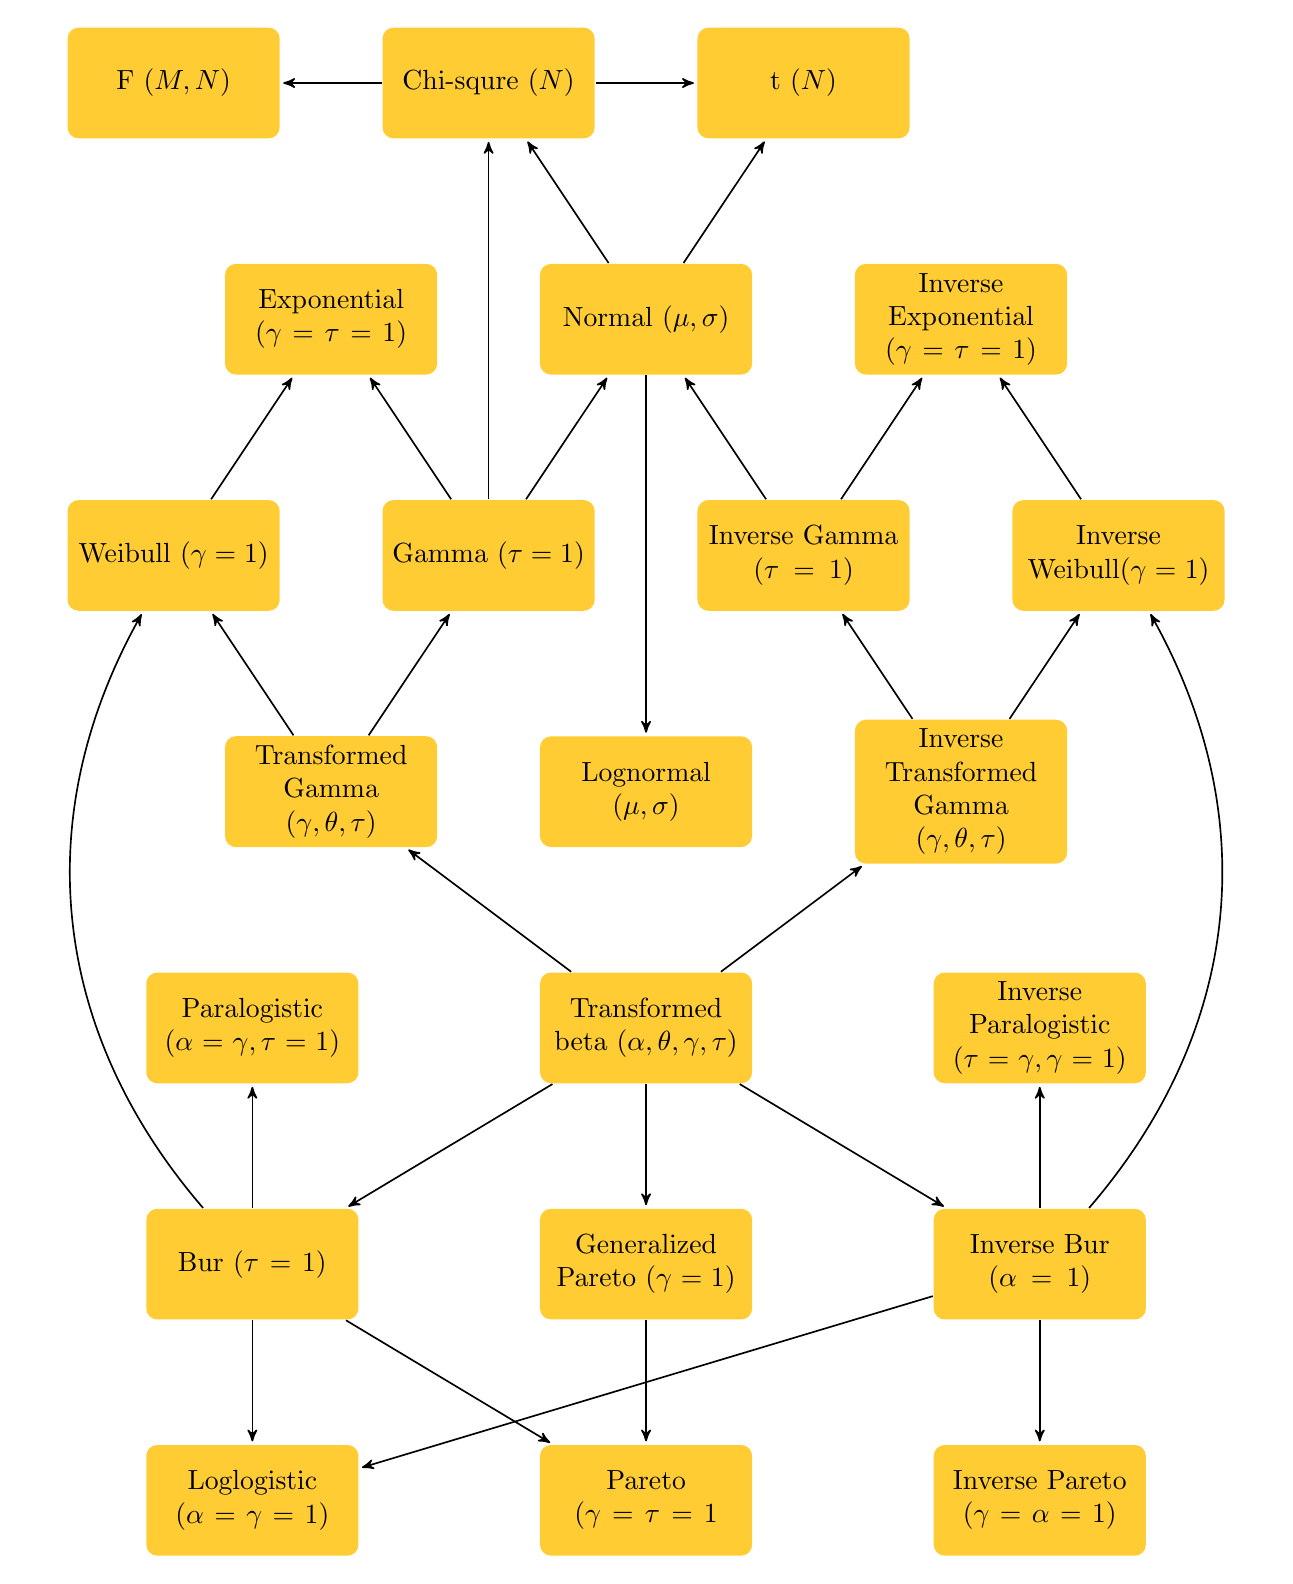
\begin{tikzpicture}[->,>=stealth',shorten >=1pt,auto,node distance=2.8cm,
                    semithick]
  \tikzstyle{every state}=[rectangle,fill=yellow1,draw=none,text=black, text width=7em,text centered,rounded corners, minimum height=4em]
  \node[state]         (Tb) at (0, 0)              {Transformed beta ($\alpha,\theta,\gamma,\tau$)};
  \node[state]         (GP) at (0, -3)           {Generalized Pareto ($\gamma=1$)};
  \node[state]         (P) at (0, -6)        {Pareto ($\gamma=\tau=1$};
  \node[state]         (Bu) at (-5, -3)        {Bur ($\tau=1$)};
  \node[state]         (log) at (-5, -6)        {Loglogistic ($\alpha=\gamma=1$)};
  \node[state]         (plog) at (-5, 0)        {Paralogistic ($\alpha=\gamma,\tau=1$)};
  \node[state]       (iBu) at (5, -3)        {Inverse Bur ($\alpha=1$)};
  \node[state]         (iP) at (5, -6)        {Inverse Pareto ($\gamma=\alpha=1$)};
  \node[state]         (iplog) at (5, 0)        {Inverse Paralogistic ($\tau=\gamma,\gamma=1$)};
  \node[state]         (TG) at (-4, 3)       {Transformed Gamma ($\gamma,\theta,\tau$)};
  \node[state]         (G) at (-2, 6)        {Gamma ($\tau=1$)};
  \node[state]         (W) at (-6, 6)        {Weibull ($\gamma=1$)};
  \node[state]         (E) at (-4, 9)        {Exponential ($\gamma=\tau=1$)};
  \node[state]         (iTG) at (4, 3)       {Inverse Transformed Gamma ($\gamma,\theta,\tau$)};
  \node[state]         (iG) at (2, 6)        {Inverse Gamma ($\tau=1$)};
  \node[state]         (iW) at (6, 6)        {Inverse Weibull($\gamma=1$)};
  \node[state]         (iE) at (4, 9)        {Inverse Exponential ($\gamma=\tau=1$)};
  \node[state]         (N) at (0, 9)        {Normal ($\mu,\sigma$)};
  \node[state]         (LN) at (0, 3)        {Lognormal ($\mu,\sigma$)};
  \node[state]         (Chi) at (-2, 12)        {Chi-squre ($N$)};
  \node[state]         (t) at (2, 12)        {t ($N$)};
  \node[state]         (F) at (-6, 12)        {F ($M,N$)};
  \path (Tb) edge              node {} (GP);
  \path (GP) edge              node {} (P);
  \path (Tb) edge              node {} (Bu);
  \path (Bu) edge              node {} (log);
  \path (Bu) edge              node {} (P);
  \path (Bu) edge              node {} (plog);
  \path (iBu) edge              node {} (log);
  \path (iBu) edge              node {} (iP);
  \path (iBu) edge              node {} (iplog);
  \path (Tb) edge              node {} (iBu);
  \path (Tb) edge              node {} (TG);
  \path (TG) edge              node {} (G);
  \path (TG) edge              node {} (W);
  \path (G) edge              node {} (E);
  \path (W) edge              node {} (E);
  \path (Tb) edge              node {} (iTG);
  \path (iTG) edge              node {} (iG);
  \path (iTG) edge              node {} (iW);
  \path (iG) edge              node {} (iE);
  \path (iW) edge              node {} (iE);
  \path (N) edge              node {} (LN);
  \path (G) edge              node {} (N);
  \path (iG) edge              node {} (N);
  \path (Bu) edge[bend left=35]    node {} (W);
  \path (iBu) edge[bend right=35]     node {} (iW);
  \path (G) edge   node {} (Chi);
  \path (N) edge   node {} (Chi);
  \path (Chi) edge   node {} (t);
  \path (Chi) edge   node {} (F);
  \path (N) edge   node {} (t);
\end{tikzpicture}
\end{center}
\subsubsection{Beta distribution family}
The PDF and CDF of Transformed Beta distribution



The PDF and CDF of Beta distribution (the commonly used version)  are:
$$
f(x;\alpha,\beta)=\frac{x^{\alpha-1}(1-x)^{\beta-1}}{B(\alpha,\beta)},
\qquad
F(x;\alpha,\beta)=\frac{B(x;\alpha,\beta)}{B(\alpha,\beta)}
$$
where
$$
B(\alpha,\beta)=\int_0^1u^\alpha (1-u)^{\beta-1},
\qquad
B(x;\alpha,\beta)=\int_0^xu^\alpha (1-u)^{\beta-1}
$$
\begin{figure}[htb]
\centering
\subfigure[PDF of Beta]{
\includegraphics[height=6cm,width=8cm]{pic/betapdf.pdf}}
\subfigure[CDF of Beta]{
\includegraphics[height=6cm,width=8cm]{pic/betacdf.pdf}}
\caption{Beta distribution}
\end{figure}


\section{Estimate}

\section{Prove}




\end{document}
